\documentclass[a4paper,11pt]{article}
\usepackage{dmasproject}

% if you need additional LaTeX packages, add them here

\title{Anime Character Generation}
% sort your names alphabetically by last name
\author{
  Wenjie Zhang (5677291) ~~
  Qi Le (5674954) ~~
  John Dunlap (5354238)   
}
% \date{Alpha version, September 2020} % change this accordingly

\begin{document}

\maketitle

\section{Introduction}
In this project, we use Generative Adversarial Networks (GANs \cite{goodfellow2014generative}) to generate anime pictures.
We choose WGAN-div as our basic model, which leverages Wasserstein divergence as its loss function. Comparing the 64*64 resolution pictures generated from WGAN-div (figure \ref{fig:append-a-01}) to the 128*128 resolution pictures generated from WGAN-div (figure \ref{fig:append-a-02}), we could find a little improvement in the imaging quality. But in general, the imaging quality is not very good.

\section{Background and Challenges}
At first, our team wanted to implement the StyleGAN2 by ourselves after learning the source code posted by NVIDIA. Then we realized that it was not applicable for two reasons. The first reason is that the project itself is very complicated and we do not have enough optimization knowledge for reproducing the project. The second reason is that the Anime Character Generation might not need the high-resolution picture to show the details of the faces. Thus, we decided to implement a simpler model first and then add some modules that we learned from the StyleGAN2 project to our model to improve the image quality.

We selected WGAN-div as our basic model from DCGAN, WGAN, WGAN-GP, LSGAN, SNGAN. Compared to DCGAN, WGAN-div has a better loss function – Wasserstein divergence, which is a smooth function.

For traditional GANs (e.g. DCGAN), the generator tries to minimize the following loss function (while the discriminator tries to maximize it):

\begin{equation}
    \begin{aligned}
    % \max_G \min_D
    loss = -\mathbb{E}_{x\sim P_r}[\log D(x)] - \mathbb{E}_{x\sim P_g}[\log(1-D(G(z)))]
    \end{aligned}
\end{equation}

In this function, $D(x)$ is the discriminator's estimate of the probability that real data instance x is real.
G(z) is the generator's output when given noise z, and D(G(z)) is the discriminator's estimate of the probability that a fake instance is real.
By taking its derivative with respect to $D$ as 0, we can get

\begin{equation}
    \begin{aligned}
    D^*(x) = \frac{P_r(x)}{P_r(x) + P_g(x)}
    \end{aligned}
\end{equation}

Denote that $KL(P_1||P_2) = \mathbb{E}_{x \sim P_1} \log \frac{P_1}{P_2}$, we have
\begin{equation}
    \begin{aligned}
    JS(P_1 || P_2) &= \frac{1}{2}KL(P_1||\frac{P_1 + P_2}{2}) + \frac{1}{2}KL(P_2||\frac{P_1 + P_2}{2})
    \end{aligned}
    \label{eq:gan-dist-kl}
\end{equation}

Then we can obtain that
\begin{equation}
    \begin{aligned}
    loss = 2JS(P_r || P_g) - 2\log 2
    \end{aligned}
\end{equation}

When the discriminator is trained too well, the generator gradient disappears (i.e. $\nabla \rightarrow$ 0), thus the generator loss cannot be reduced. When the discriminator is not well trained, the generator gradient is not accurate. We need to balance between training the discriminator too well and not well, which is in fact very difficult for GANs.

\begin{equation}
    \begin{aligned}
    W(P_r, P_g) = \inf_{\gamma \sim \Pi (P_r, P_g)} \mathbb{E}_{(x, y) \sim \gamma} [||x - y||]
    \end{aligned}
    \label{eq:wgan-dist}
\end{equation}

% In a short way, traditional GANs choose to classify instances.
Wasserstein GANs does not directly classify instances, however, it outputs the their distance (equation \ref{eq:wgan-dist}). When the $P_r$ and $P_g$, especially at the beginning, do not effectively overlap, $KL$ and $JS$ in equation \ref{eq:gan-dist-kl} is nearly 0, but the Wasserstein distance can still reflect their difference. In other words, there will a be more smooth gradient in WGANs.
Of course, WGAN is also challenging, and we are still working on it.


\section{Implementation and Discussion}
The goal of our project is to improve the quality of the generated images. By now, there are two ways in front of us. The first way is to improve the resolution of the input and generated pictures. With the increasing resolution of the pictures, more and more details would show up on the generated pictures. The second way is the main focus of our group. We are trying to add some modules learned from the StyleGAN2 to our basic WGAN-div models. StyleGAN2 has 4 main changes in the new style-based generator:
\begin{itemize}
    \item Removing traditional input. (figure \ref{fig:append-b-01})
    \item Mapping Network. (figure \ref{fig:append-b-02})
    \item Style modules (AdaIN). (figure \ref{fig:append-b-03})
    \item Stochastic variation (Stochastic variation, generates random details for the generator by adding noise). (figure \ref{fig:append-b-04})
\end{itemize}
We want to add the first three parts to the WGAN-div model in the next steps and see how the generated pictures would change.

For the rest of the semester, we are working on improving our generated pictures to have more details and clearer parts on the faces (e.g. figure \ref{fig:result-expect}). Further, we are working on optimizing our work to make the generated pictures be close to the pictured generated from the StyleGAN2 model above.
\begin{figure}[htb]
    \centering
    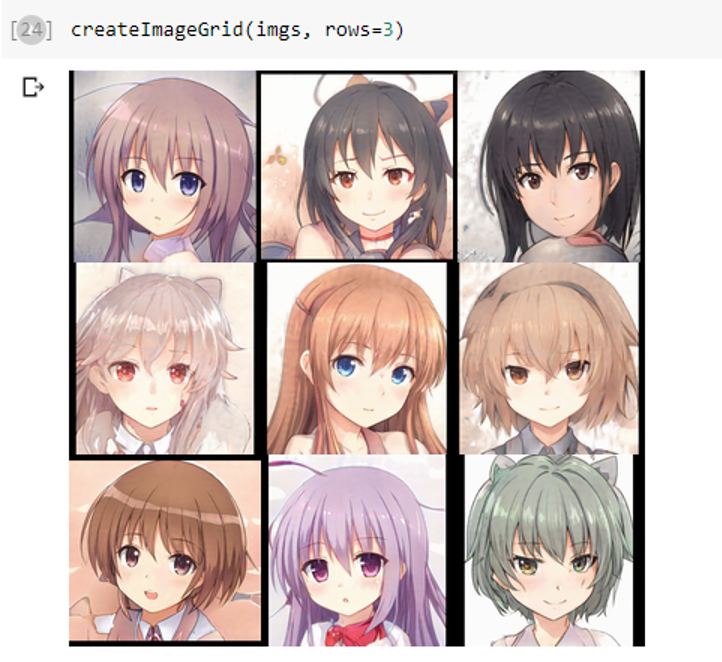
\includegraphics[width=0.5\linewidth]{figure/result-expect.png}
    \caption{Pictures generated from StyleGAN2 model.}
    \label{fig:result-expect}
\end{figure}


% This will print you references, please do not change it.
\printbibliography

\appendix
\section{Appended Results}
\begin{figure}[htb]
    \centering
    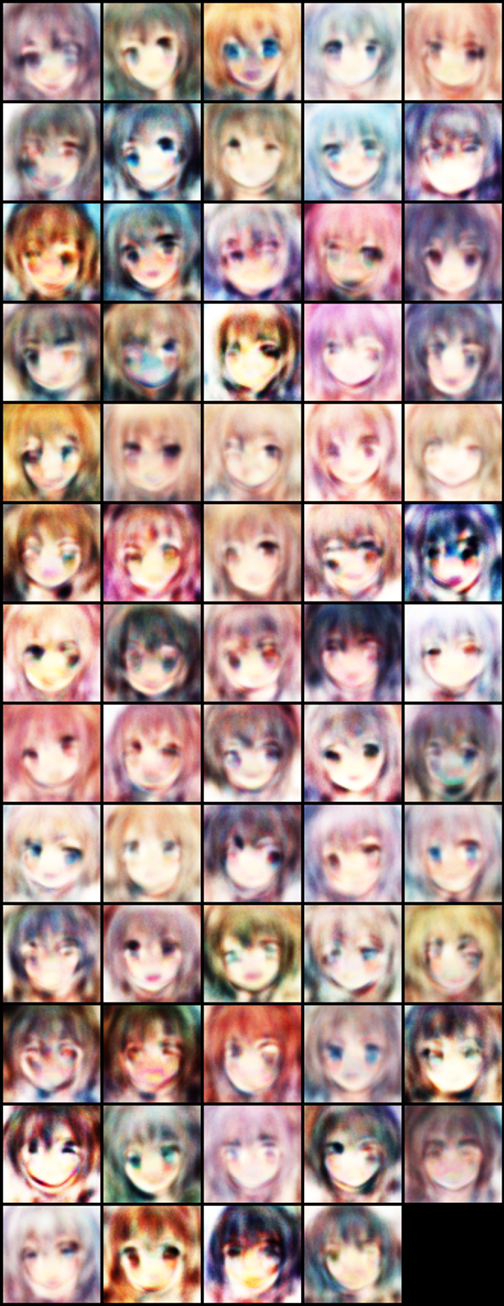
\includegraphics[width=0.3\linewidth]{figure/append-a-01.png}
    \caption{64*64 resolution pictures generated from the WGAN-div.}
    \label{fig:append-a-01}
\end{figure}

\begin{figure}[htb]
    \centering
    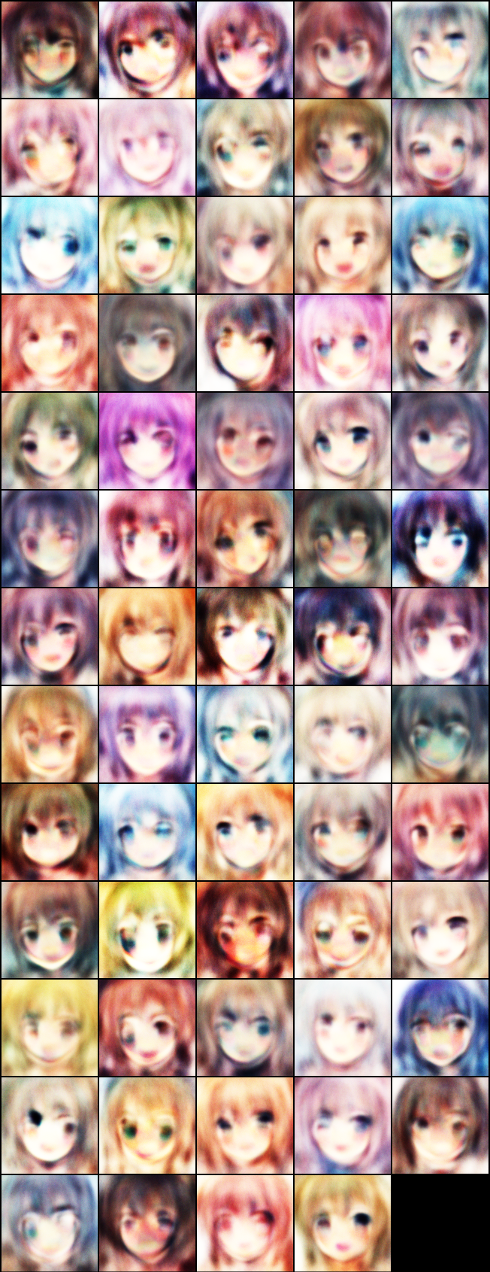
\includegraphics[width=0.3\linewidth]{figure/append-a-02.png}
    \caption{128*128 resolution pictures generated from the WGAN-div.}
    \label{fig:append-a-02}
\end{figure}

% \section{Appended Models}
\begin{figure}[htb]
    \centering
    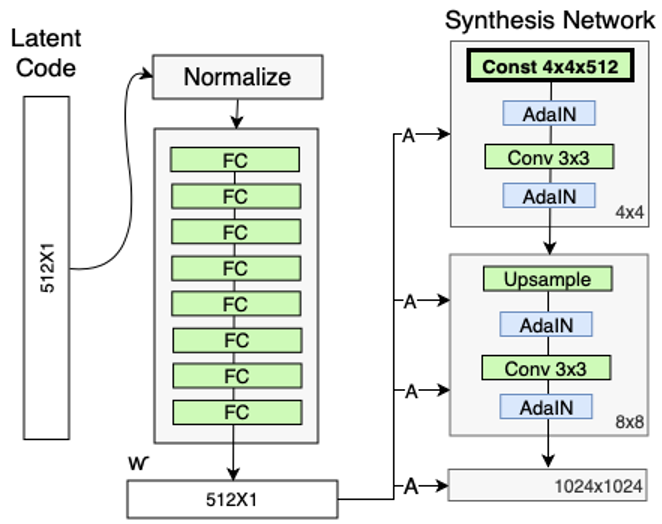
\includegraphics[width=0.5\linewidth]{figure/append-b-01.png}
    \caption{The Synthesis Network input is replaced with a constant input \cite{horev2018style}}
    \label{fig:append-b-01}
\end{figure}

\begin{figure}[htb]
    \centering
    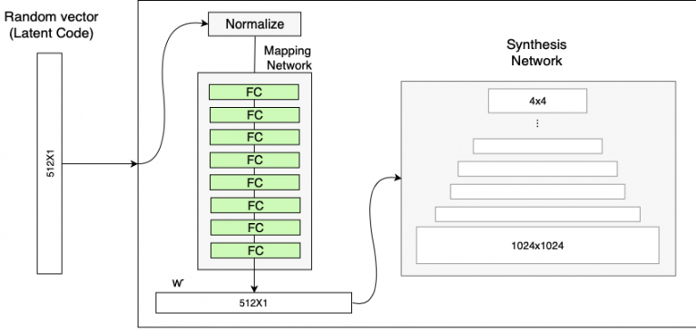
\includegraphics[width=0.6\linewidth]{figure/append-b-02.png}
    \caption{The generator with the Mapping Network (in addition to the ProGAN synthesis network) \cite{horev2018style}}
    \label{fig:append-b-02}
\end{figure}

\begin{figure}[htb]
    \centering
    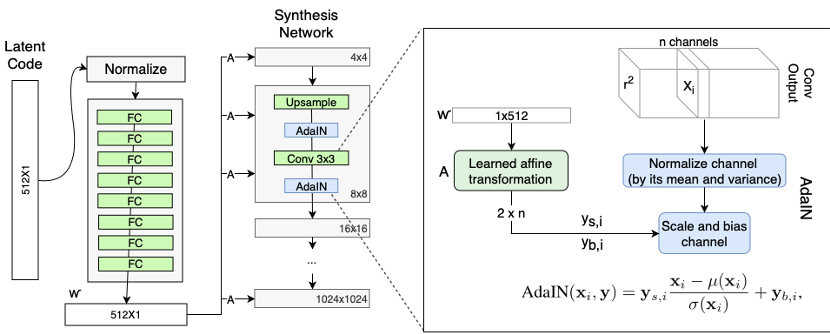
\includegraphics[width=0.8\linewidth]{figure/append-b-03.png}
    \caption{The generator’s Adaptive Instance Normalization (AdaIN) \cite{horev2018style}}
    \label{fig:append-b-03}
\end{figure}


\begin{figure}[htb]
    \centering
    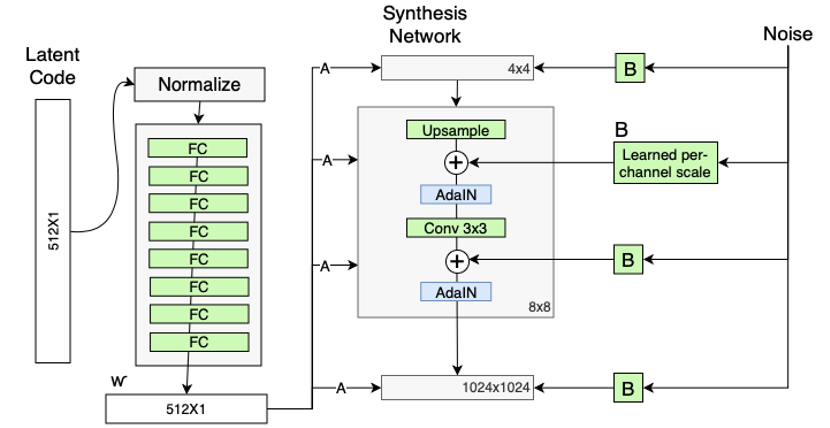
\includegraphics[width=0.7\linewidth]{figure/append-b-04.png}
    \caption{Adding scaled noise to each resolution level of the synthesis network \cite{horev2018style}}
    \label{fig:append-b-04}
\end{figure}

\end{document}
